\section{DNS}

\subsection{Opgave 1}
\begin{figure}[H]
	\centering
	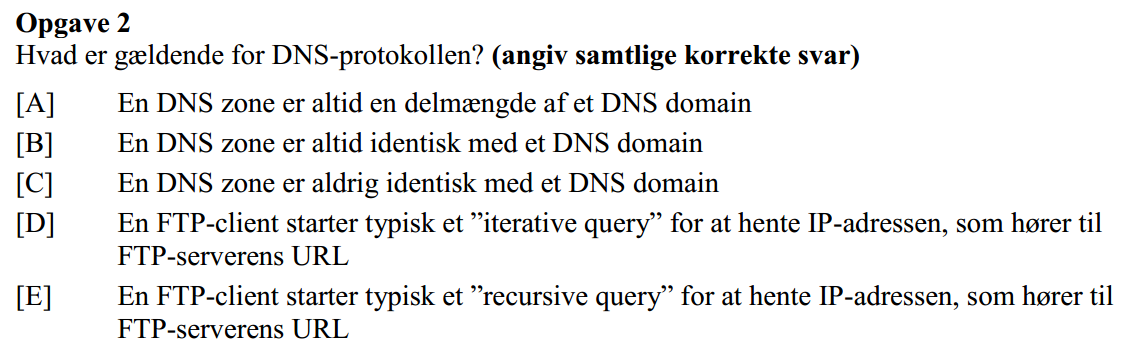
\includegraphics[width=\linewidth]{figs/dns/SE15OP2}
\end{figure}

\paragraph{[A]}
En DNS zone er altid en delmængde. En zone kan indeholde sub-domæner af et hoveddomæne.

\paragraph{[E]}
En iterativ DNS query vil resultere i at DNS serveren ikke sender et definitivt svar men derimod sender en reference til den DNS server som har svaret.

En recursivt DNS query vil derimod resultere i at den kontaktede DNS server har ansvaret for at finde næste server. 
